\chapter{State of the Art}
\label{chap:state-of-the-art}

\lettrine[lines=3, findent=3pt, nindent=0pt]{T}{his} chapter rounds out the theoretical background and technologies used in the project and discussed in the following: beginning with how network traffic is made ad how to characterize malicious activities, it will then be discussed Software Defined Networking as an industry standard and then \gls{ml} will be introduced, with particular emphasis on Intrusion Detection applications of \textit{Deep Learning}. The reader should here be provided with sufficient knowledge to understand chapters \ref{chap:methodology}, \ref{chap:results} and \ref{chap:conclusions}.

%----------------------------------------------------
% NETWORK TRAFFIC
%----------------------------------------------------

\section{Network Traffic}
\label{sec:network-traffic}

\textit{Network Traffic} is the amount of data that passes through a network at a given time, and it represents the starting point to the project. \\ Network architecture was thought to be modular and explicit, to ensure that modifications made to a single component were transparent to the rest of the system. This modularization is represented by \textit{network protocols} being separated into different layers: each layer has a precise task. In 1960s the \textit{U.S. Department of Defense} designed the \textit{TCP/IP} model, which is now the \textit{de facto} standard for protocols stack. Network security should be addressed at each TCP/IP network layer for different vulnerabilities and attack types \cite{Zaman2009}.

\begin{figure}[h!]
    \centering
    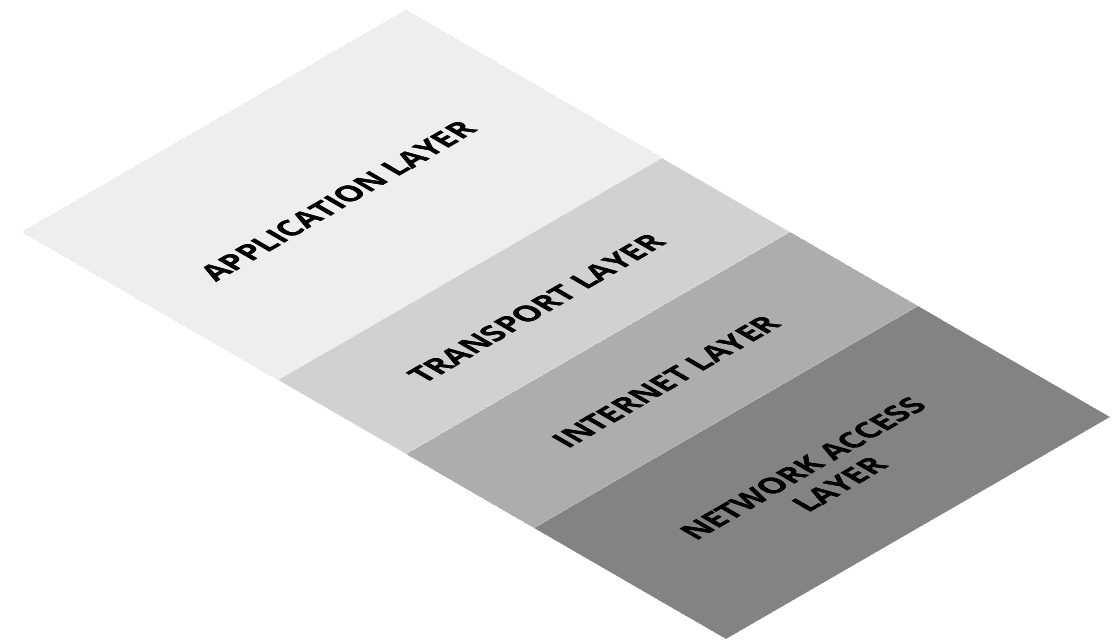
\includegraphics[scale=0.23]{figures/TCP_IP Stack.png}
    \caption{Internet protocol suite: TCP/IP Stack}
    \label{fig:TCP/IP-stack}
\end{figure}

TCP/IP stack is composed of 4 layers, representing from the physical connection (\textit{Network Access Layer}) to the user interface (\textit{Application Layer}). \\ The most relevant layer for this project is the third one: \textit{Transport Layer}, also called \textit{Host to Host Layer} is responsible for end-to-end communication and error-free delivery of data. It shields the upper-layer applications from the complexities of data. The main protocols used in this layer are:

\begin{itemize}
    \item[\faCaretRight] \gls{tcp}: provides reliable and error-free communication between end systems. It also has acknowledgement features and a flow control system. This protocol has a lot of overhead due to its features;
    \item[\faCaretRight] \gls{udp}: unlikely \gls{tcp}, this protocol doesn't ensure a reliable connection between points, but it is very cost effective and lightweight.
\end{itemize}
Network packets are encapsulated in either a \textit{TCP segment} or a \textit{UDP datagram}. Another relevant protocol that will be used is \gls{icmp}, belonging to the second layer (\textit{Internet Layer}): it s responsible for providing hosts with information about network problems. Because of the particular design of network architecture, in which one layer acts as an intermediate between the layer above and the one below, when trying to characterize the traffic, looking only at these latter protocols can be sufficient \cite{Iglesias2015}.

%----------------------------------------------------
% SOFTWARE DEFINED NETWORKING
%----------------------------------------------------

\subsection{Software Defined Networking}
\label{subsec:sdn}

Follows a brief introduction on \gls{sdn} as an industry standard, now widely available also in consumer-grade equipment. These notions will be useful to comprehend section \ref{subsec:traffic-characterization}. \\
\gls{sdn} technology is an approach to network management that enables dynamic and efficient network configuration with the aim of improving network performance and monitoring. It was first issued by \gls{ietf} in the 2000s and since its refinement it was associated with \textit{OpenFlow protocol}, although nowadays it isn't anymore an exclusive solution. In the \gls{sdn} paradigm the network architecture consists fo three planes: \textit{data plane} (that forwards traffic according to the decisions made by the control plane), \textit{control plane} (that decides how to handle network traffic) and \textit{application plane} \cite{Kreutz2015}.

\begin{figure}[h!]
    \centering
    \begin{tikzpicture}[scale=.55,every node/.style={minimum size=1cm},on grid]
            
        %slanting: production of a set of n 'laminae' to be piled up. N=number of grids.
        \begin{scope}[
                yshift=-83,every node/.append style={
                yslant=0.5,xslant=-1},yslant=0.5,xslant=-1
                ]
            % opacity to prevent graphical interference
            \fill[white,fill opacity=0.9] (0,0) rectangle (5,5);
            \draw (2.5,2.5) node {\fontsize{50}{60} \faRandom};
            \draw[black,very thick] (0,0) rectangle (5,5);%marking borders
            %Idem as above, for the n-th grid:
        \end{scope}
            
        \begin{scope}[
            yshift=0,every node/.append style={
                yslant=0.5,xslant=-1},yslant=0.5,xslant=-1
                         ]
            \fill[white,fill opacity=.9] (0,0) rectangle (5,5);
            \draw[black,very thick] (0,0) rectangle (5,5);
            \draw (2.5,2.5) node {\fontsize{50}{60} \faServer};
        \end{scope}
            
        \begin{scope}[
            yshift=90,every node/.append style={
            yslant=0.5,xslant=-1},yslant=0.5,xslant=-1
                         ]
            \fill[white,fill opacity=.9] (0,0) rectangle (5,5);
            \draw (2.5,2.5) node {\fontsize{50}{60} \faTv};
            \draw[black,dashed] (0,0) rectangle (5,5);
        \end{scope}
    
        %putting arrows and labels:
        \draw[-latex,thick] (6,4) node[right]{$\mathsf{Control\; Plane}$}
             to[out=180,in=90] (3.5,2.5);
    
        \draw[-latex,thick](6,1)node[right]{$\mathsf{Data\; Plane}$}
             to[out=180,in=90] (3.5,-0.5);
    
        \draw[-latex,thick](6,7)node[right]{$\mathsf{Application\; Plane}$}
            to[out=180,in=90] (3.5,5.5);
        
    \end{tikzpicture}
    \caption{\gls{sdn} paradigm}
    \label{fig:sdn-paradigm}
\end{figure}
The bottom plane is made up of \gls{sdn}-enabled switches, that send routing request to the above plane, instead of calculating routing rules by themselves when receiving new \textit{flows}, then the control plane calculates paths for the requests and assigns the routing rules in compliance with the applications in the top plane \cite{Xu2017}. A \textit{flow} is a sequence of packets with the same values for \textit{source ip}, \textit{destination ip}, \textit{source port}, \textit{destination port} and \textit{protocol} \cite{icissp17}. The \textit{controller} exercises direct control over the state in the data plane elements via well-defined \glsplural{api}, such as OpenFlow. An OpenFlow switch has one or more tables of packet-handling rules (flow table). Each rule matches a subset of the traffic and performs certain actions on the traffic. Depending on the rules installed by a controller application, an OpenFlow switch can - instructed by the controller - behave like a router, switch, firewall, or perform other roles and this is the meaning of \textit{Software Defined} in \gls{sdn}.

%----------------------------------------------------
% SOFTWARE DEFINED NETWORKING
%----------------------------------------------------

\subsubsection{SDN Controller}
\label{ssubsec:sdn-controller}

%See paper \cite{Zhu2019} and \cite{Bondkovskii2016} \\
The \textit{controller} in the control plane is the fundamental element used for all operations of data plane management. Hence, the performance and capabilities of the controller itself are extremely important and in this project its \glsplural{api} will be needed for building a network traffic monitor (and such data will be use to recognize any possible attack). In \cite{Bondkovskii2016} and \cite{Zhu2019} different controllers are compared based on benchmarks, programming languages, documentation and other parameters (\textit{Northbound \glsxtrshort{api}}, \textit{Southbound \glsxtrshort{api}}, \textit{Multithreading}, \textit{Modularity}, etc). \\ In light of this, the controller of choice for the project will be \textit{Ryu Controller}: it outperformed other controllers on almost every benchmark, it has a very well made documentation \cite{RyuDoc} and it supports OpenFlow protocol up to version 1.5.

%----------------------------------------------------
% TRAFFIC CHARACTERIZATION
%----------------------------------------------------

%See paper \cite{Iglesias2015}, \cite{Sharafaldin2019} and \cite{icissp17} and \cite{Xu2017} and \cite{Dainotti2006} and \cite{Wijesinghe2015}

\subsection{Traffic Characterization}
\label{subsec:traffic-characterization}

Anomaly detection in communication networks provides the basis for uncovering misconfigurations, network failures and potential threats. Resource and time constraints create the need of restricting to a limited number of features the traffic characterization and task detection. Limiting the resources spent for the observation and the analysis of such data, also improves the quality of the detection, since trivial and redundant data will not be considered. There are two different methodologies to characterize network traffic: \textit{packet inspection} and \textit{flow-based characterization}. The first one consists of inspecting each network packet; it is very resource consuming and not always allowed since the payload can be encrypted. On the other hand, the second one is less precise, but much more cost effective and lightweight \cite{Alaidaros2017}. Machine learning methodologies can improve the detection rate of \textit{flow-based characterization} \cite{Iglesias2015}: this makes it a reliable go-to. In \cite{icissp17} \textit{time-related} features are suggested to characterize traffic with ease:
\begin{itemize}
    \item[\faCaretRight] \textit{Active}: duration of sending packets before idle;
    \item[\faCaretRight] \gls{biat}: time between two packets sent backward;
    \item[\faCaretRight] \textit{Duration}: duration of the considered flow.
    \item[\faCaretRight] \gls{fbpsec}: bytes sent per second in either direction;
    \item[\faCaretRight] \gls{flowiat}: time between two packets sent in either direction; 
    \item[\faCaretRight] \gls{fppsec}: packets sent per second in either direction;
    \item[\faCaretRight] \gls{fiat}: time between two packets sent forward; 
    \item[\faCaretRight] \textit{Idle}: amount of time the flow was idling before becoming active;
\end{itemize}
For all the features (extracted using \textit{Ryu Controller}) also the respective mean, minimum, maximum and standard deviation are calculated and so can be considered as features-groups. \\
\lipsum[1-3]

%----------------------------------------------------
% MALICIOUS TRAFFIC
%----------------------------------------------------

\subsection{Malicious Network Traffic}
\label{subsec:malicious-traffic}

An \textit{intrusion} can be defined as an attempt to access information about computer systems or to damage system operation in an illegal or unauthorized manner \cite{Liu2019}, hence it will be considered \textit{malicious traffic} the entirety of network traffic generated by such operations. \\
The classes of malicious traffic analyzed in this work are the following:

\begin{itemize}
    \item[\faCaretRight] \textit{Botnet}: a botnet is a number of Internet connected devices, used to perform various tasks, from stealing data, to spam, or to practice \gls{ddos} attacks. Automated infection tools can also be used to scan for and compromise suitable zombie systems \cite{icissp18} and \cite[p.~250]{Sharafaldin2019};
    \item[\faCaretRight] \textit{Bruteforce}: this kind of attack is one of the most popular and it can be used to guess passwords or \glsxtrshortpl{url} (in order to discover hidden contents in web applications). It can be defined as an hint and try attack, that corresponds of trying every possible key on a piece of ciphertext until an intelligible translation into plaintext is obtained \cite{icissp18} and \cite[p.~43]{Sharafaldin2019};
    \item[\faCaretRight] \gls{xss}: this kind of vulnerability can typically be found in web applications. An \gls{xss} attack consist of injecting client-side scripts into \glsxtrshort{html} content of web pages, that can be viewed by other users and aims to gain elevated access privileges to sensitive data belong- ing to other sites \cite[p.~387]{Sharafaldin2019};
    \item[\faCaretRight] \gls{dos}: the objective of this attack is to exhaust some critical resources associated with the target service, denying or preventing legitimate users to access the system or the network \cite[p.~241]{Sharafaldin2019};
    \item[\faCaretRight] \gls{ddos}: unlike the previous type of attack, the incoming traffic flooding the victim is obtained from many different sources. This effectively makes it impossible to stop the attack simply by blocking a single source and guarantees much more bandwidth to the attacker \cite[p.~241]{Sharafaldin2019};
    \item[\faCaretRight] \textit{Heartbleed}: this particular attack exploits a bug in the OpenSSL cryptography library, widely used implementation of the \gls{tls} protocol. It was discovered in 2014 and allowed to expose significant amounts of memory on the vulnerable system \cite{Carvalho2014}, \cite{icissp18}, \cite{Stallings2014} and \cite[p.~706]{Sharafaldin2019};
    \item[\faCaretRight] \textit{Port Scanning}: this occurs when an attacker sends probe packets to gather intelligence information about the infrastructure, based on the responses received \cite{icissp18};
    \item[\faCaretRight] \gls{sqli}: it is one of the most prevalent and dangerous network-based security threats that uses malicious database queries to extract bulk data from the latter; this can occur, for example, through badly projected forms on web pages \cite[p.~163]{Sharafaldin2019}.
\end{itemize}
This list isn't exhaustive of all possible network violations, but these are the attacks contained in the dataset\footnote{See section \ref{subsec:datasets-for-evaluation}} used for the evaluation. Regarding the characterization of said violations, a comprehensive list of network features and related attacks can be found in appendix \ref{app:net-features}.

%----------------------------------------------------
% INTRUSION DETECTION SYSTEMS
%----------------------------------------------------

\section{Intrusion Detection Systems}
\label{sec:intrusion-detection-system}

\lipsum[1-4]

    \begin{figure}[h!]
        \centering
        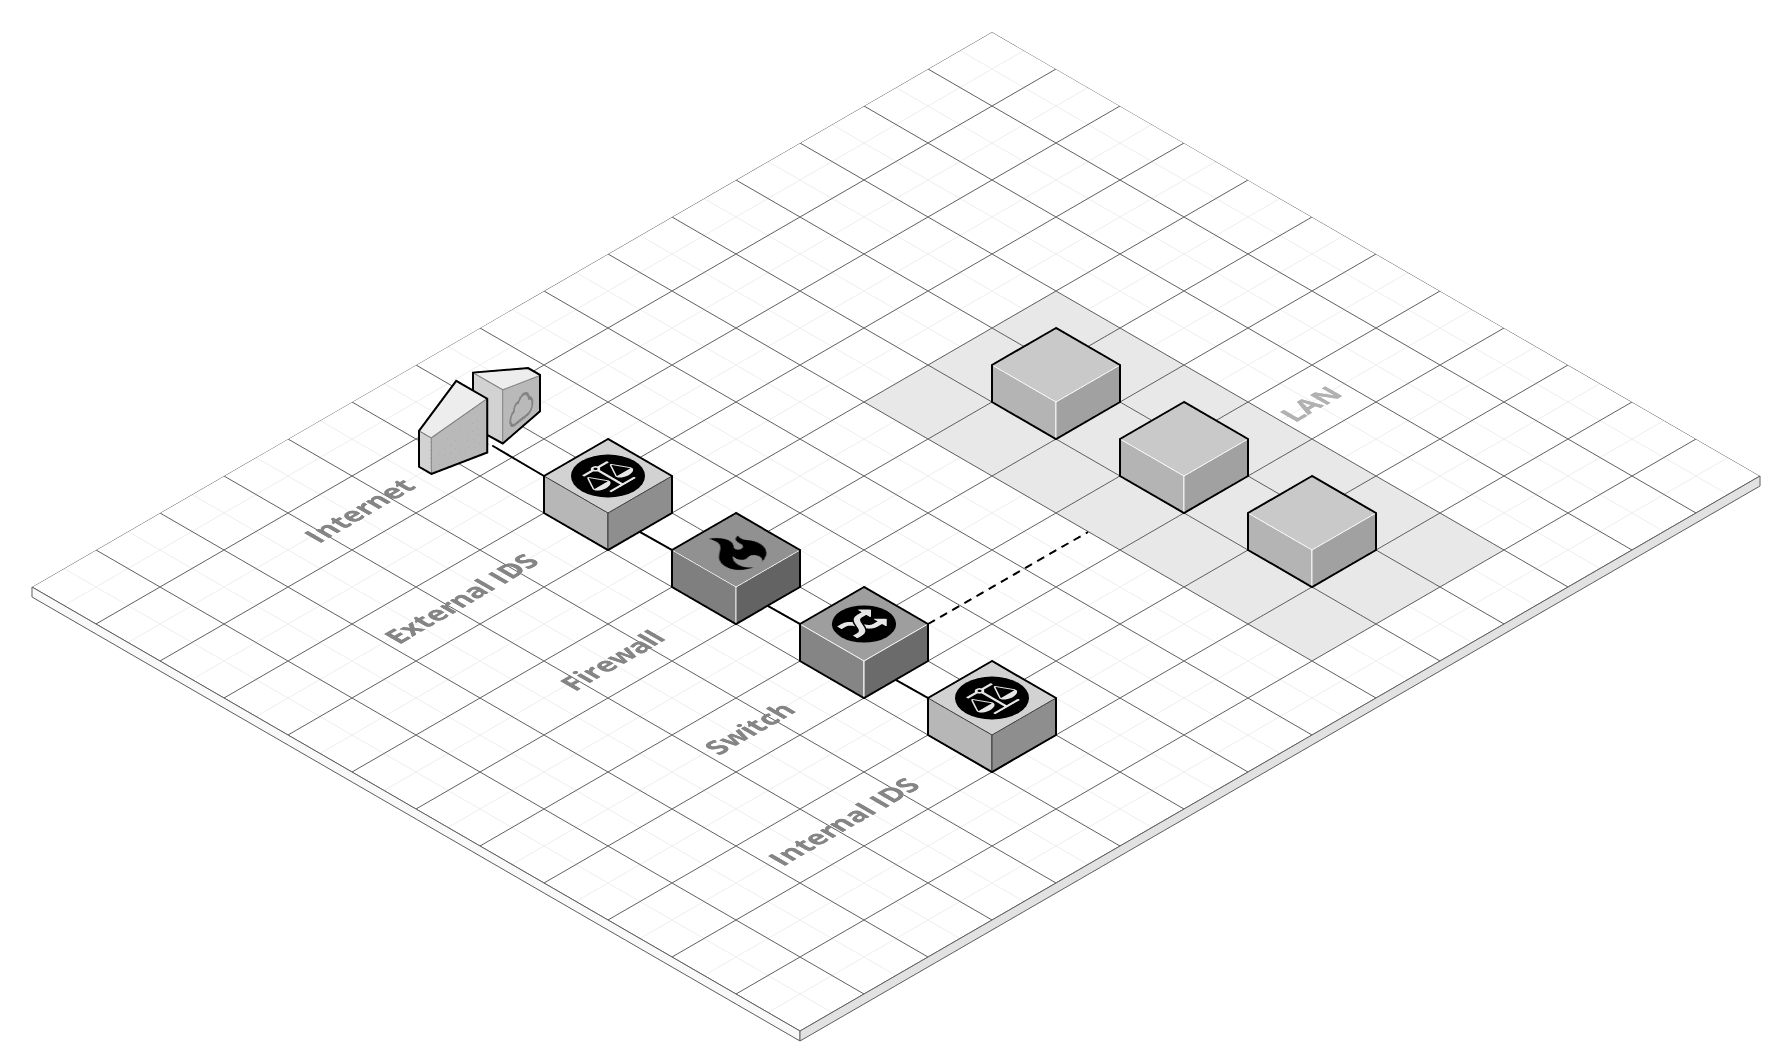
\includegraphics[scale=0.23]{figures/Intrusion Detection System Model.png}
        \caption{Intrusion Detection System Model}
        \label{fig:IDS-model}
    \end{figure}

%----------------------------------------------------
% DETECTION RATES
%----------------------------------------------------

\subsection{Detection rates}

See paper bla bla

%----------------------------------------------------
% TAXONOMY OF INTRUSION DETECTION SYSTEMS
%----------------------------------------------------

\subsection{Taxonomy of Intrusion Detection Systems}

See paper \cite{Liu2019}

%----------------------------------------------------
% DATASETS FOR INTRUSION DETECTION SYSTEMS
%----------------------------------------------------

\subsection{Datasets for Intrusion Detection Evaluation}
\label{subsec:datasets-for-evaluation}

See paper \cite{icissp18}, \cite{Khraisat2019} and \cite{Leevy2020} \\

\lipsum[1-6]

\begin{center}
    \begin{chronology}[5]{1983}{2010}{\textwidth}
        \event{1984}{One}
        \event[1985]{1986}{two}
        \event{\decimaldate{25}{12}{2001}}{three}
    \end{chronology}
\end{center}

%----------------------------------------------------
% MACHINE LEARNING
%----------------------------------------------------

\section{Machine Learning}
\label{sec:machine-learning}

See paper \cite{Khraisat2019} and \cite{Hodo2017} \\

\lipsum \\
Discussed in \ref{sec:machine-learning}

%----------------------------------------------------
% MACHINE LEARNING ALGORITHMS
%----------------------------------------------------

\subsection{Machine Learning Algorithms}
\label{subsec:ml-algorithms}

\lipsum

%----------------------------------------------------
% DEEP LEARNING
%----------------------------------------------------

\subsection{Deep Learning}
\label{subsec:deep-learning}

\lipsum

%----------------------------------------------------
% MACHINE LEARNING LIBRARIES
%----------------------------------------------------

\subsection{Machine Learning Libraries}
\label{subsec:ml-libraries}

\lipsum[1-5]